\documentclass[tikz,border=0pt]{standalone}
\pdfminorversion=7
\usepackage[T1]{fontenc}
\usepackage{lmodern,amsmath,amssymb,graphicx}
\usepackage{pgfplots}
\usetikzlibrary{arrows.meta,calc,positioning,patterns,decorations.pathreplacing}
\pgfplotsset{compat=1.18}
\definecolor{family}{RGB}{0,140,18}
\definecolor{familypale}{RGB}{225,255,226}
\definecolor{frozen}{RGB}{49,57,208}
\definecolor{frozenpale}{RGB}{234,235,255}
\definecolor{adapter}{RGB}{219,102,0}
\definecolor{adapterpale}{RGB}{255,196,135}
\definecolor{outputcol}{RGB}{120,38,130}
\definecolor{ink}{RGB}{33,33,33}
\definecolor{muted}{RGB}{105,105,105}
\tikzset{
 figure/.style={x=1pt,y=1pt,line cap=round,line join=round,text=ink,
   >={Stealth[length=7pt,width=6pt]},font=\fontsize{20}{24}\selectfont},
 title/.style={font=\fontsize{29}{33}\selectfont},
 heading/.style={font=\fontsize{22}{26}\selectfont},
 labeltext/.style={font=\fontsize{18}{22}\selectfont,align=center},
 smalllabel/.style={font=\fontsize{15}{19}\selectfont,align=center},
 equation/.style={font=\fontsize{24}{29}\selectfont,align=center},
 flow/.style={->,line width=1.3pt},
 fineflow/.style={->,line width=.8pt},
 target/.style={circle,fill=family,draw=white,line width=1.2pt,inner sep=0pt,minimum size=12pt},
 candidate/.style={circle,fill=white,draw=muted,line width=1.3pt,inner sep=0pt,minimum size=10pt},
 neuron/.style={circle,draw=frozen,fill=frozen!18,minimum size=13pt,inner sep=0pt,line width=.8pt}
}
\DeclareMathOperator{\rank}{rank}
\DeclareMathOperator{\row}{row}
\DeclareMathOperator{\col}{col}
\newcommand{\R}{\mathbb R}
\graphicspath{{assets/}}
\newcommand{\canvas}[1]{\path[use as bounding box] (0,0) rectangle (960,600);
  \node[title,anchor=west] at (36,557) {#1};}
\newcommand{\glyphgrid}[2]{
 \begin{scope}[shift={(#1,#2)}]
  \fill[white] (0,0) rectangle (136,136);
  \foreach \x/\y/\c in {1/1/80,2/2/80,2/3/45,3/4/45,3/5/45,4/5/100,4/6/45,5/6/45,5/4/45,5/2/100,6/1/80}{
    \fill[frozen!\c] (\x*17,\y*17) rectangle ++(17,17);
  }
  \draw[step=17pt,black!30,line width=.35pt] (0,0) grid (136,136);
  \draw[black!45,line width=.6pt] (0,0) rectangle (136,136);
 \end{scope}}

\begin{document}
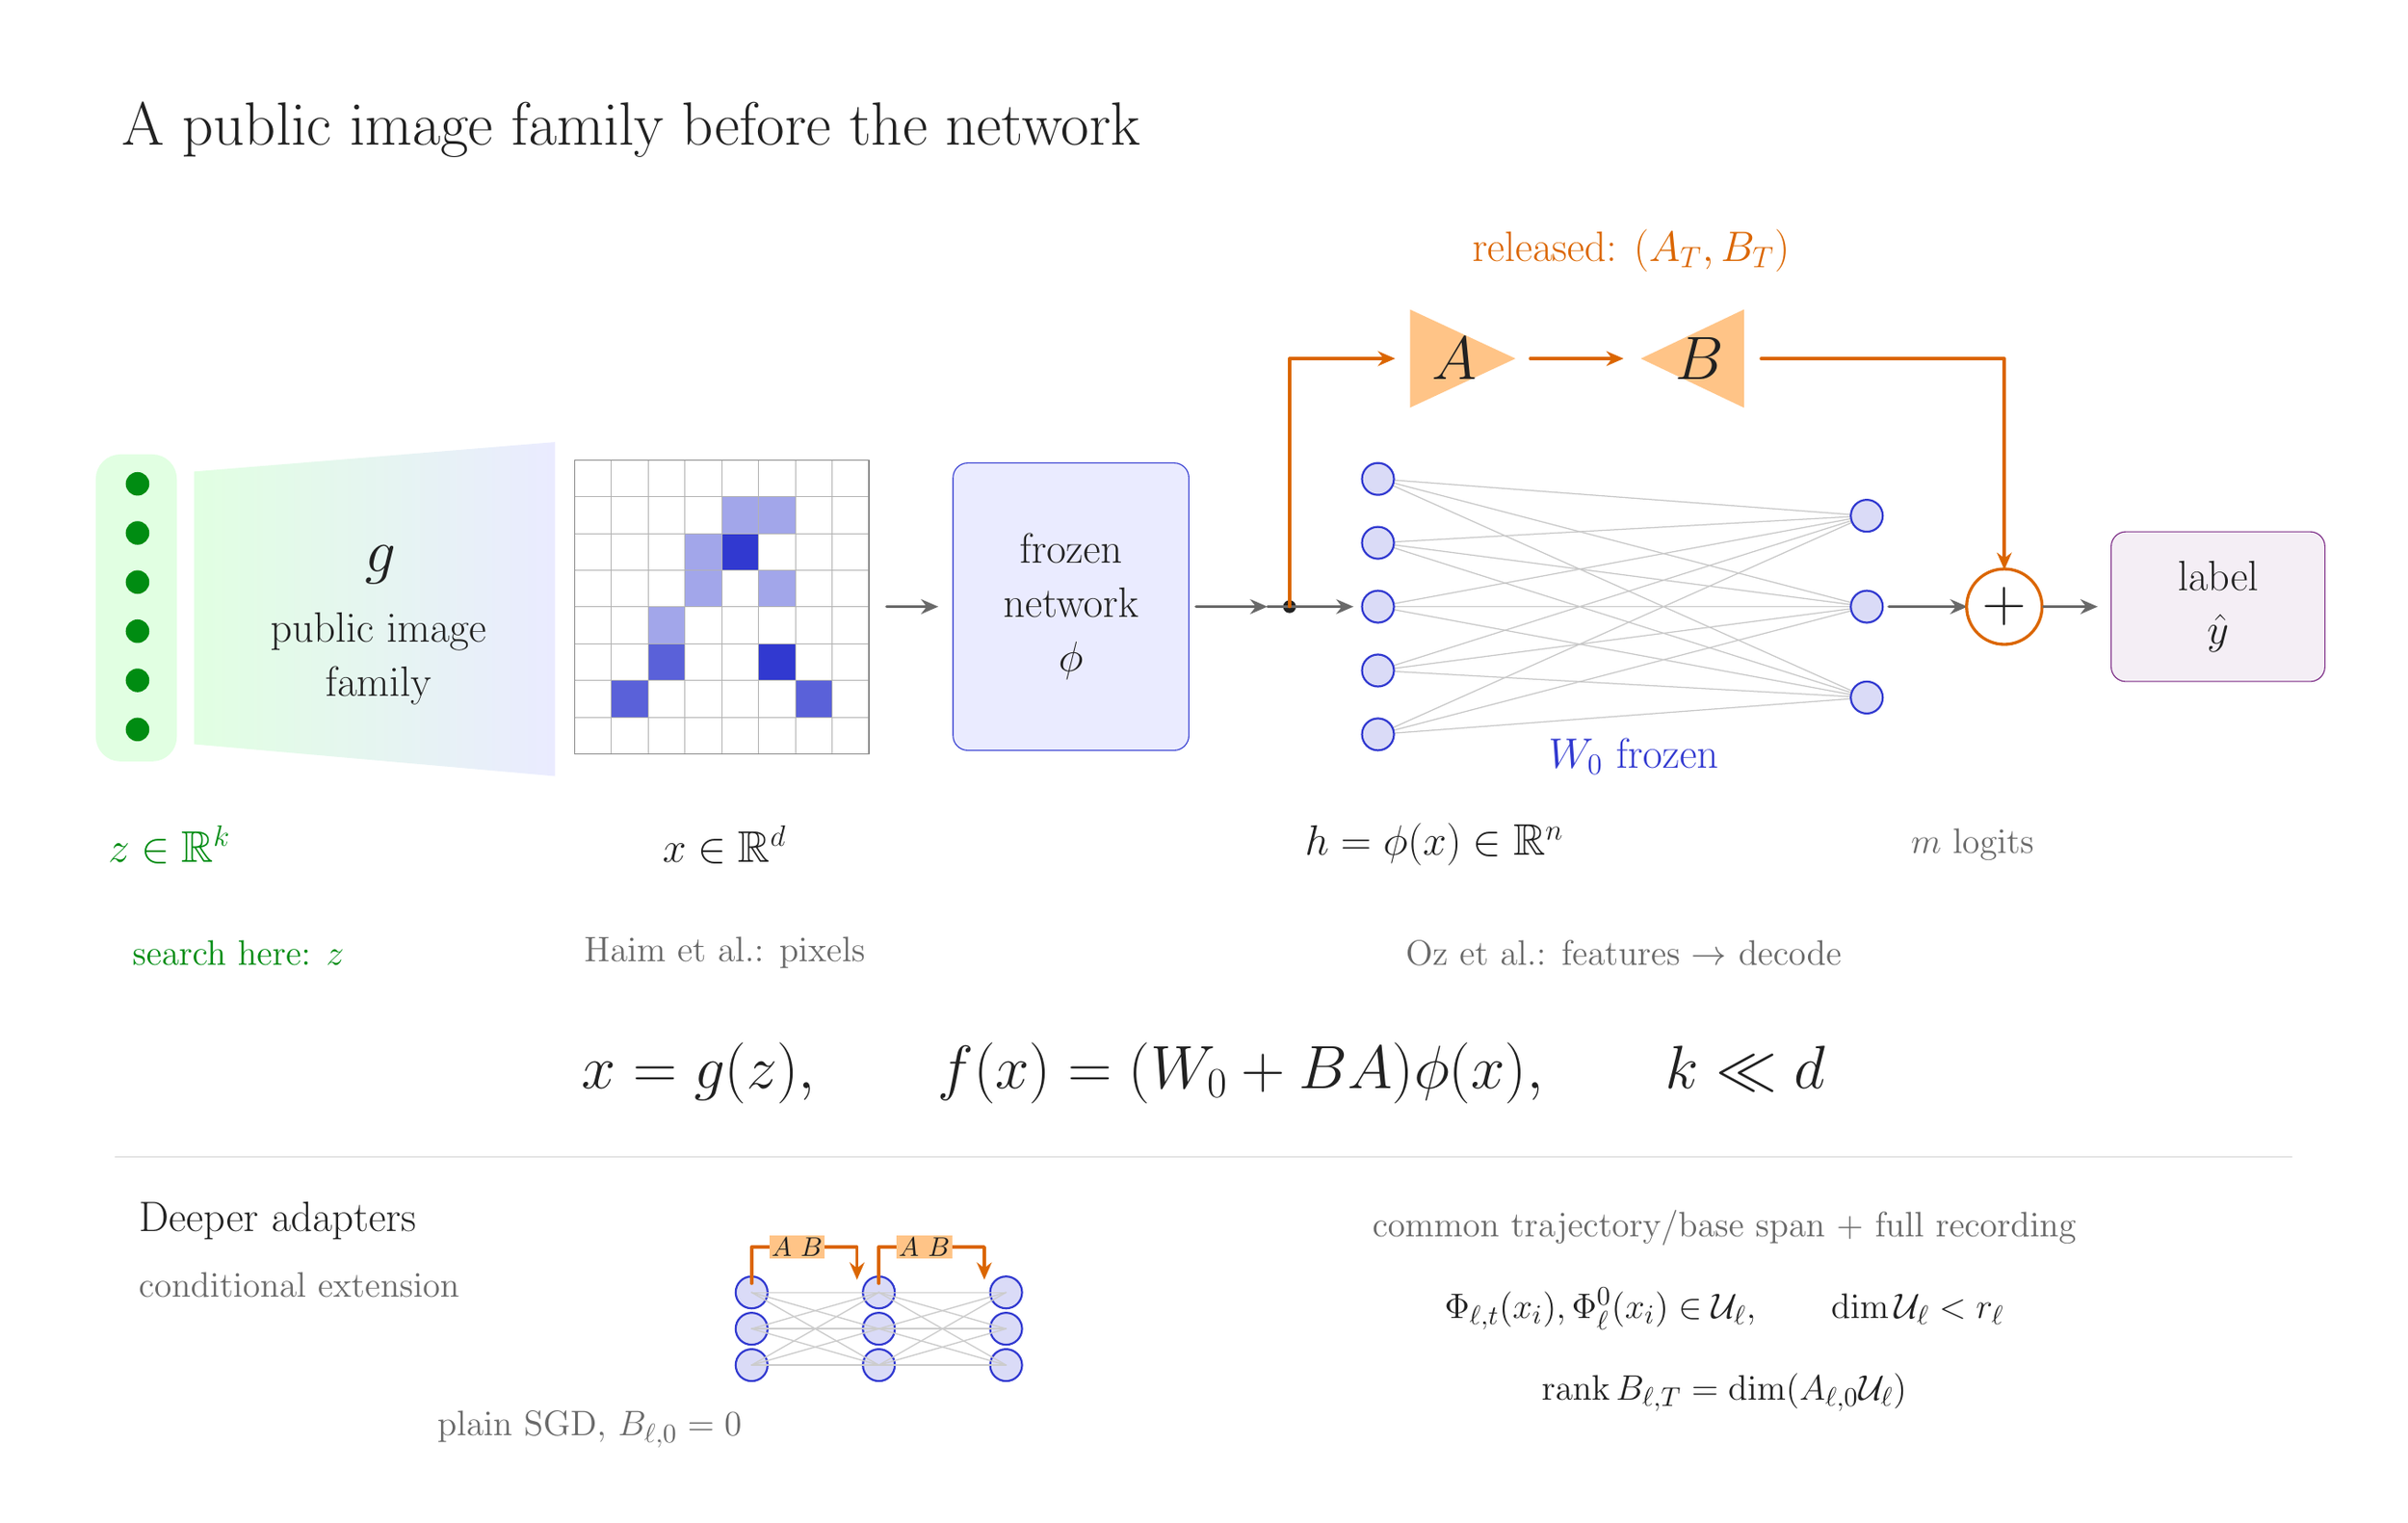
\begin{tikzpicture}[figure]
\canvas{A public image family before the network}
\fill[familypale,rounded corners=10pt] (29,300) rectangle (62,425);
\foreach \y in {313,333,353,373,393,413} \fill[fill=family] (46,\y) circle (4.8pt);
\shade[left color=familypale,right color=frozenpale] (69,307)--(216,294)--(216,430)--(69,418)--cycle;
\node[equation] at (145,380) {$g$};
\node[labeltext] at (144,342) {public image\\family};
\begin{scope}[shift={(224,303)},scale=.88]\glyphgrid{0}{0}\end{scope}
\draw[flow,muted] (351,363)--(372,363);
\node[draw=frozen,fill=frozenpale,rounded corners=6pt,minimum width=96pt,minimum height=117pt,
      labeltext] at (426,363) {frozen\\network\\$\phi$};
\draw[flow,muted] (477,363)--(506,363);
\fill[ink] (515,363) circle (2.6pt);
\draw[fineflow,muted] (506,363)--(541,363);
\foreach \y in {311,337,363,389,415} {
  \foreach \v in {326,363,400} \draw[black!22,line width=.45pt] (551,\y)--(750,\v);
  \node[neuron] at (551,\y) {};
}
\foreach \y in {326,363,400} \node[neuron] at (750,\y) {};
\node[labeltext,text=frozen] at (655,302) {$W_0$ frozen};
\draw[flow,adapter] (515,363)--(515,464)--(558,464);
\fill[adapterpale] (564,444)--(564,484)--(607,464)--cycle;
\node[equation] at (582,464) {$A$};
\draw[flow,adapter] (613,464)--(651,464);
\fill[adapterpale] (700,444)--(700,484)--(658,464)--cycle;
\node[equation] at (682,464) {$B$};
\draw[flow,adapter] (707,464)--(806,464)--(806,378);
\node[labeltext,text=adapter] at (654,508) {released: $(A_T,B_T)$};
\draw[flow,muted] (759,363)--(791,363);
\node[circle,draw=adapter,line width=1.2pt,inner sep=2.5pt,font=\fontsize{25}{28}\selectfont] at (806,363) {$+$};
\draw[flow,muted] (822,363)--(844,363);
\node[draw=outputcol,fill=outputcol!8,rounded corners=6pt,minimum width=87pt,
      minimum height=61pt,labeltext] at (893,363) {label\\$\hat y$};
\node[labeltext,text=family] at (59,266) {$z\in\R^k$};
\node[labeltext] at (285,266) {$x\in\R^d$};
\node[labeltext] at (574,266) {$h=\phi(x)\in\R^n$};
\node[smalllabel,text=muted] at (793,266) {$m$ logits};
\node[smalllabel,text=family] at (87,222) {search here: $z$};
\node[smalllabel,text=muted] at (285,222) {Haim et al.: pixels};
\node[smalllabel,text=muted] at (651,222) {Oz et al.: features $\to$ decode};
\node[equation] at (480,173) {$x=g(z),\qquad f(x)=(W_0+BA)\phi(x),\qquad k\ll d$};
\draw[black!18,line width=.65pt] (37,139)--(923,139);
\node[labeltext,anchor=west] at (43,113) {Deeper adapters};
\node[smalllabel,text=muted,anchor=west] at (43,87) {conditional extension};
\begin{scope}[shift={(296,69)},scale=.74]
  \foreach \x in {0,70,140} {
    \foreach \y in {-20,0,20} \node[neuron] at (\x,\y) {};
  }
  \foreach \a in {-20,0,20} \foreach \b in {-20,0,20} {
    \draw[black!20,line width=.5pt] (0,\a)--(70,\b);
    \draw[black!20,line width=.5pt] (70,\a)--(140,\b);
  }
  \foreach \x in {0,70} {
    \draw[flow,adapter] (\x,25)--(\x,45)--(\x+58,45)--(\x+58,27);
    \node[fill=adapterpale,font=\fontsize{11}{13}\selectfont,inner sep=1pt] at (\x+25,45) {$A\ B$};
  }
\end{scope}
\node[smalllabel,text=muted] at (692,110) {common trajectory/base span $+$ full recording};
\node[smalllabel] at (692,77) {$\Phi_{\ell,t}(x_i),\Phi^0_\ell(x_i)\in\mathcal U_\ell,\qquad\dim\mathcal U_\ell<r_\ell$};
\node[smalllabel] at (692,43) {$\rank B_{\ell,T}=\dim(A_{\ell,0}\mathcal U_\ell)$};
\node[smalllabel,text=muted] at (230,28) {plain SGD, $B_{\ell,0}=0$};
\end{tikzpicture}
\end{document}
